\chapter{Adaptive Beamforming Background}
\label{chap:abf_background}

\section{Introduction}

In this section, the concept of beamforming, and its method of adaptation, is introduced. It's assumed the reader is familiar with fundamental discrete signal processing techniques, such as Finite Impulse Response (FIR) filtering.

\section{Beamforming}

In signal processing, filtering is a fairly common operation; in the discrete sense, samples are passed through a set of filter coefficients, or "taps", to perform the convolution and acheive the desired response. Analagous to such temporal filtering, an array of sensors can be filtered \emph{spatially} to produce a desired response across the elements. Specifically in the context of Radio Frequency (RF) antenna arrays, this spatial filtering can be utilized to optimize the overall antenna gain pattern

Introduce your thesis \citep{Alexander_and_Ghirnikar,Haykin}

As seen in Figure \ref{fig:ula_beamformer}

\begin{figure}[!htbp]
  \centering
  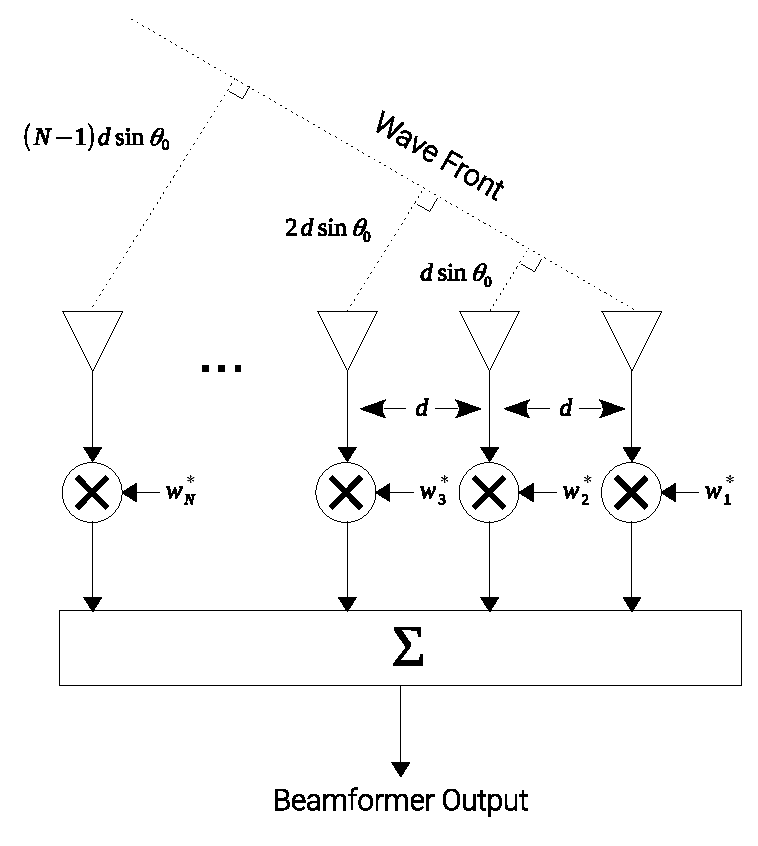
\includegraphics[]{02_abf_background/ula_beamformer}
  \caption{ULA Beamformer}
  \label{fig:ula_beamformer}
\end{figure}

\subsection{Adaptive Weight Calculation}

\subsection{QR Decomposition}

hello \citep{AN506}


%% TODO below is scratchpad for tikz stuff & tables

% example table
\begin{table}[ht]
\centering
\begin{tabular}{rr}
  \hline
A & B \\
  \hline
  1 & -0.40 \\
    2 & -1.27 \\
    3 & -1.04 \\
    4 & 0.69 \\
    5 & 0.08 \\
    6 & 1.71 \\
    7 & 1.90 \\
    8 & 1.88 \\
    9 & 0.17 \\
   10 & -1.62 \\
   \hline
\end{tabular}
\caption{\bf{ Table title } Table description}
\label{tab:rtab1}
\end{table}


\tikzset{
block/.style = {draw, fill=white, rectangle, minimum height=3em, minimum width=3em},
tmp/.style  = {coordinate},
sum/.style= {draw, fill=white, circle, node distance=1cm},
input/.style = {coordinate},
output/.style= {coordinate},
pinstyle/.style = {pin edge={to-,thin,black}
}
}

% htbp to ease floating placement https://tex.stackexchange.com/questions/2275/keeping-tables-figures-close-to-where-they-are-mentioned
\begin{figure}[!htbp]
\centering
\begin{tikzpicture}[auto, node distance=2cm,>=latex']
    \node [input, name=rinput] (rinput) {};
    \node [sum, right of=rinput] (sum1) {};
    \node [block, right of=sum1] (controller) {$k_{p\beta}$};
    \node [block, above of=controller,node distance=1.3cm] (up){$\frac{k_{i\beta}}{s}$};
    \node [block, below of=controller,node distance=1.3cm] (rate) {$sk_{d\beta}$};
    \node [sum, right of=controller,node distance=2cm] (sum2) {};
    \node [block, above = 2cm of sum2](extra){$\frac{1}{\alpha_{\beta2}}$};  %
    \node [block, right of=sum2,node distance=2cm] (system)
{$\frac{a_{\beta 2}}{s+a_{\beta 1}}$};
    \node [output, right of=system, node distance=2cm] (output) {};
    \node [tmp, below of=controller] (tmp1){$H(s)$};
    \draw [->] (rinput) -- node{$R(s)$} (sum1);
    \draw [->] (sum1) --node[name=z,anchor=north]{$E(s)$} (controller);
    \draw [->] (controller) -- (sum2);
    \draw [->] (sum2) -- node{$U(s)$} (system);
    \draw [->] (system) -- node [name=y] {$Y(s)$}(output);
    \draw [->] (z) |- (rate);
    \draw [->] (rate) -| (sum2);
    \draw [->] (z) |- (up);
    \draw [->] (up) -| (sum2);
    \draw [->] (y) |- (tmp1)-| node[pos=0.99] {$-$} (sum1);
    \draw [->] (extra)--(sum2);
    \draw [->] ($(0,1.5cm)+(extra)$)node[above]{$d_{\beta 2}$} -- (extra);
    \end{tikzpicture}
    \caption{A PID Control System}
    \label{fig:pid}
\end{figure}



% reuse from Kalman example https://texample.net/tikz/examples/kalman-filter/
\begin{figure}[htbp]
\centering
% The state vector is represented by a blue circle.
% "minimum size" makes sure all circles have the same size
% independently of their contents.
\tikzstyle{state}=[circle,
                   thick,
                   minimum size=1.2cm,
                   draw=blue!80,
                   fill=blue!20]

% The measurement vector is represented by an orange circle.
\tikzstyle{measurement}=[circle,
                         thick,
                         minimum size=1.2cm,
                         draw=orange!80,
                         fill=orange!25]

% The control input vector is represented by a purple circle.
\tikzstyle{input}=[circle,
                   thick,
                   minimum size=1.2cm,
                   draw=purple!80,
                   fill=purple!20]

% The input, state transition, and measurement matrices
% are represented by gray squares.
% They have a smaller minimal size for aesthetic reasons.
\tikzstyle{matrx}=[rectangle,
                   thick,
                   minimum size=1cm,
                   draw=gray!80,
                   fill=gray!20]

% The system and measurement noise are represented by yellow
% circles with a "noisy" uneven circumference.
% This requires the TikZ library "decorations.pathmorphing".
\tikzstyle{noise}=[circle,
                   thick,
                   minimum size=1.2cm,
                   draw=yellow!85!black,
                   fill=yellow!40,
                   decorate,
                   decoration={random steps,
                               segment length=2pt,
                               amplitude=2pt}]

% Everything is drawn on underlying gray rectangles with
% rounded corners.
\tikzstyle{background}=[rectangle,
                        fill=gray!10,
                        inner sep=0.2cm,
                        rounded corners=5mm]

\begin{tikzpicture}[>=latex,text height=1.5ex,text depth=0.25ex]
  % "text height" and "text depth" are required to vertically
  % align the labels with and without indices.

  % The various elements are conveniently placed using a matrix:
  \matrix[row sep=0.5cm,column sep=0.5cm] {
    % First line: input sample array
        \node (other_in0)  {$\vdots$}; &
        \node (other_in1)  {$\vdots$}; &
        \node (other_in2)  {$\vdots$}; &
        \node (other_in3)  {$\vdots$}; &
        \\
        \node (t2_in0)  {$x(2)$}; &
        \node (t2_in1)  {$x(1)$}; &
        \node (t2_in2)  {$x(0)$}; &
        \node (t2_in3)  {$d(2)$}; &
        \\
        \node (t1_in0)  {$x(1)$}; &
        \node (t1_in1)  {$x(0)$}; &
        \node (t1_in2)  {$0$};    &
        \node (t1_in3)  {$d(1)$}; &
        \\
        \node (t0_in0)  {$x(0)$}; &
        \node (t0_in1)  {$0$};    &
        \node (t0_in2)  {$0$};    &
        \node (t0_in3)  {$d(0)$}; &
        \\
    % First line: Control input
    &
        \node (u_k-1) [input]{$\mathbf{u}_{k-1}$}; &
        &
        \node (u_k)   [input]{$\mathbf{u}_k$};     &
        &
        \node (u_k+1) [input]{$\mathbf{u}_{k+1}$}; &
        \\
        % Second line: System noise & input matrix
        \node (w_k-1) [noise] {$\mathbf{w}_{k-1}$}; &
        \node (B_k-1) [matrx] {$\mathbf{B}$};       &
        \node (w_k)   [noise] {$\mathbf{w}_k$};     &
        \node (B_k)   [matrx] {$\mathbf{B}$};       &
        \node (w_k+1) [noise] {$\mathbf{w}_{k+1}$}; &
        \node (B_k+1) [matrx] {$\mathbf{B}$};       &
        \\
        % Third line: State & state transition matrix
        \node (A_k-2)         {$\cdots$};           &
        \node (x_k-1) [state] {$\mathbf{x}_{k-1}$}; &
        \node (A_k-1) [matrx] {$\mathbf{A}$};       &
        \node (x_k)   [state] {$\mathbf{x}_k$};     &
        \node (A_k)   [matrx] {$\mathbf{A}$};       &
        \node (x_k+1) [state] {$\mathbf{x}_{k+1}$}; &
        \node (A_k+1)         {$\cdots$};           \\
        % Fourth line: Measurement noise & measurement matrix
        \node (v_k-1) [noise] {$\mathbf{v}_{k-1}$}; &
        \node (H_k-1) [matrx] {$\mathbf{H}$};       &
        \node (v_k)   [noise] {$\mathbf{v}_k$};     &
        \node (H_k)   [matrx] {$\mathbf{H}$};       &
        \node (v_k+1) [noise] {$\mathbf{v}_{k+1}$}; &
        \node (H_k+1) [matrx] {$\mathbf{H}$};       &
        \\
        % Fifth line: Measurement
        &
        \node (z_k-1) [measurement] {$\mathbf{z}_{k-1}$}; &
        &
        \node (z_k)   [measurement] {$\mathbf{z}_k$};     &
        &
        \node (z_k+1) [measurement] {$\mathbf{z}_{k+1}$}; &
        \\
    };

    % The diagram elements are now connected through arrows:
    \path[->]
        (A_k-2) edge[thick] (x_k-1)	% The main path between the
        (x_k-1) edge[thick] (A_k-1)	% states via the state
        (A_k-1) edge[thick] (x_k)		% transition matrices is
        (x_k)   edge[thick] (A_k)		% accentuated.
        (A_k)   edge[thick] (x_k+1)	% x -> A -> x -> A -> ...
        (x_k+1) edge[thick] (A_k+1)

        (x_k-1) edge (H_k-1)				% Output path x -> H -> z
        (H_k-1) edge (z_k-1)
        (x_k)   edge (H_k)
        (H_k)   edge (z_k)
        (x_k+1) edge (H_k+1)
        (H_k+1) edge (z_k+1)

        (v_k-1) edge (z_k-1)				% Output noise v -> z
        (v_k)   edge (z_k)
        (v_k+1) edge (z_k+1)

        (w_k-1) edge (x_k-1)				% System noise w -> x
        (w_k)   edge (x_k)
        (w_k+1) edge (x_k+1)

        (u_k-1) edge (B_k-1)				% Input path u -> B -> x
        (B_k-1) edge (x_k-1)
        (u_k)   edge (B_k)
        (B_k)   edge (x_k)
        (u_k+1) edge (B_k+1)
        (B_k+1) edge (x_k+1)
        ;

    % Now that the diagram has been drawn, background rectangles
    % can be fitted to its elements. This requires the TikZ
    % libraries "fit" and "background".
    % Control input and measurement are labeled. These labels have
    % not been translated to English as "Measurement" instead of
    % "Messung" would not look good due to it being too long a word.
    \begin{pgfonlayer}{background}
        \node [background,
                    fit=(w_k-1) (v_k-1) (A_k+1)] {};
        \node [background,
                    fit=(z_k-1) (z_k+1),
                    label=left:Measure:] {};
    \end{pgfonlayer}
\end{tikzpicture}

\caption{Kalman filter system model}
\end{figure}
